\subsection{Curve Sketching}\label{subsec-curve-sketching}

\begin{definition}\label{def-local-minimum-maximum}
	A point $x_0$ is called a local minimum if $f(x) \geq f(x_0)$ for all $x$ in
	a neighborhood of $x_0$. Likewise, it is called a local maximum if $f(x) \geq f(x_0)$
	for all $x$ in a neighborhood of $x_0$.
\end{definition}

\begin{definition}\label{def-extrema}
	We will call $x_0$ a local extrema if $x_0$ is a local minimum or maximum.
\end{definition}

\begin{definition}\label{def-critical-point}
	We will call $x_0$ a critical point if $f^\prime(x_0)=0$ or $f$ is not differentiable
	at $x_0$.
\end{definition}

\begin{thm}\label{thm-first-derivative-test}
	Let $x_0$ be a critical point of $f$, and assume that $f$ is continuous at $x_0$
	and differentiable in a neighborhood of $x_0$, although possibly not differentiable
	at $x_0$ itself. Then the first derivative test states that
	\begin{enumerate}
		\item if $f^\prime(x_0)$ changes signs from minus to plus, then
		      $x_0$ is local minimum.
		\item if $f^\prime(x_0)$ changes signs from plus to minus, then
		      $x_0$ is local maximum.
		\item if $f^\prime(x_0)$ does not change signs, then $x_0$ is not an
		      extremum.
	\end{enumerate}
\end{thm}

\begin{thm}\label{thm-second-derivative-test}
	Let $x_0$ be a critical point of $f$, and assume that $f$ is differentiable twice
	at $x_0$. Then the second derivative test states that
	\begin{enumerate}
		\item if $f''(x_0)>0$, then $x_0$ is local minimum.
		\item if $f''(x_0)<0$, then $x_0$ is local maximum.
		\item if $f''(x_0)=0$, then this theorem doesn't reveal any additional
		      information about $x_0$
	\end{enumerate}
\end{thm}

\begin{thm}\label{thm-darboux-theorem}
	Let $f$ be a differentiable function on $[a,b]$ (with one-sided derivatives
	at the points of this interval, \textit{i.e.} $f_+^\prime(a)$ and $f_-^\prime(b)$
	exists) and let $c$ be value between $f_+^\prime(a)$ and $f_-^\prime(b)$.
	Then Darboux theorem\footnote{This is sort of an
		\hyperref[thm-intermediate-value-theorem]{intermediate value theorem}
		for derivatives.} states that there exists an $x_0$ such that $f'(x_0)=c$.
\end{thm}

\begin{crl}\label{crl-darboux-theorem}
	If $f$ is differentiable on $[a,b]$, then $f'$ may have points of infinite
	discontinuities (as they were defined in definition (\ref{def-infinite-discontinuity})).
\end{crl}

\begin{rem}\label{rem-darboux-theorem}
	The derivative of $f$ never can have removable or jump discontinuities without
	violating \hyperref[thm-darboux-theorem]{Darboux theorem}.
\end{rem}

\begin{exm}
	Consider the function
	\begin{equation*}
		f(x)=\begin{cases}
			\abs{x}^\frac{3}{2}\sin\left(\frac{1}{x}\right)\text{ if }x\neq0 \\
			0\text{ else }
		\end{cases}
	\end{equation*}
	Show that $f'$ is not continuous at $x=0$.
	\begin{flushleft}
		\textbf{Answer}: TODO
	\end{flushleft}
\end{exm}

\begin{thm}\label{thm-lhopitals-rule}
	Let $f$ and $g$ be two differentiable functions in a neighborhood of $x=a$,
	although possibly not in the neighborhood of $x$ itself. Assume that
	\begin{equation*}
		\lim_{x \to a}f(x)=\lim_{x \to a}g(x)=0
	\end{equation*}
	and that $g'(x)\neq0$ for all $x \neq a$ near $a$. Assume further that the limit
	\begin{equation*}
		\lim_{x \to a}\frac{f'(x)}{g'(x)}
	\end{equation*}
	exists. If all these conditions are met, then L'H{\^o}pital's rule says that
	\begin{equation}
		\lim_{x \to a}\frac{f(x)}{g(x)}=\lim_{x \to a}\frac{f'(x)}{g'(x)}
	\end{equation}
\end{thm}

\begin{rem}\label{rem-lhopitals-rule}
	In L'H{\^o}pital's rule we find many theorems bundled together that allow us
	under certain conditions to calculate limits of the form \enquote{$\tfrac{\infty}{\infty}$}
	or \enquote{$\tfrac{0}{0}$}.
\end{rem}

\begin{exm}\label{exm-lhopitals-rule:1}
	Consider the function $f(x)=\tfrac{\sin(x)}{x}$. Find the limit of $f$ as $x\to0$.
	\begin{flushleft}
		\textbf{Answer}: By \pref{theorem}{thm-lhopitals-rule} we get that
		\begin{align*}
			\lim_{x\to0}\frac{\sin(x)}{x} & = \lim_{x\to0}\frac{\cos(x)}{1} \\
			                              & = 1
		\end{align*}
	\end{flushleft}
	Note that this was much easier to find than in \pref{example}{exm-important-sin-over-x-limit}.
\end{exm}

\begin{exm}\label{exm-lhopitals-rule:2}
	Consider the function $f(x)=\tfrac{\ln(x)}{x-1}$. Find the limit of $f$ as $x\to1$.
	\begin{flushleft}
		\textbf{Answer}: By \pref{theorem}{thm-lhopitals-rule} we get that
		\begin{align*}
			\lim_{x\to1}\frac{\ln(x)}{x-1} & = \lim_{x\to1}\frac{\frac{1}{x}}{1} \\
			                               & = 1
		\end{align*}
	\end{flushleft}
\end{exm}

\begin{exm}\label{exm-lhopitals-rule:3}
	Consider the function $f(x)=\tfrac{\sin(x)-x}{\tan(x)-x}$. Find the limit of $f$ as $x\to0$.
	\begin{flushleft}
		\textbf{Answer}: By \pref{theorem}{thm-lhopitals-rule} we get that
		\begin{align*}
			\lim_{x\to0}\frac{\sin(x)-x}{\tan(x)-x} & = \lim_{x\to0}\frac{\cos(x)-1}{\frac{1}{\cos^2(x)}}                      \\
			                                        & = \lim_{x\to0}\frac{-\sin(x)}{-2\cdot\frac{1}{\cos^3(x)}\cdot(-\sin(x))} \\
			                                        & = -\frac{1}{2}
		\end{align*}
	\end{flushleft}
\end{exm}

\begin{exm}\label{exm-lhopitals-rule:4}
	Consider the function $f(x)=x\ln(x)$. Find the limit of $f$ as $x\to0^+$.
	\begin{flushleft}
		\textbf{Answer}: By \pref{theorem}{thm-lhopitals-rule} we get that
		\begin{align*}
			\lim_{x\to0^+}x^x & = \lim_{x\to0^+}\frac{\ln(x)}{\frac{1}{x}}         \\
			                  & = \lim_{x\to0^+}\frac{\frac{1}{x}}{-\frac{1}{x^2}} \\
			                  & = \lim_{x\to0^+}\left(-x\right)                    \\
			                  & = 0
		\end{align*}
	\end{flushleft}
\end{exm}

\begin{exm}\label{exm-lhopitals-rule:5}
	Consider the function $f(x)=x^x$. Find the limit of $f$ as $x\to0^+$.
	\begin{flushleft}
		\textbf{Answer}: By \pref{theorem}{thm-lhopitals-rule} we get that
		\begin{align*}
			\lim_{x\to0^+}x^x & = \lim_{x\to0^+}e^{\ln\left(x^x\right)}                                                  \\
			                  & = \lim_{x\to0^+}e^{x\ln(x)}             &  & \text{example (\ref{exm-lhopitals-rule:4})} \\
			                  & = 1
		\end{align*}
	\end{flushleft}
\end{exm}

\begin{definition}\label{def-convex-concave-functions}
	A function is called convex on $I$ if for all $x,y\in I$ the secant connecting
	the point $(x,f(x))$ to the point $(y,f(y))$ is above the graph. Conversely,
	a function is called concave if for all $x,y\in I$ the secant connecting
	the point $(x,f(x))$ to the point $(y,f(y))$ is below the graph.
\end{definition}

\begin{thm}\label{thm-convex-concave-first-derivative}
	Let $f$ be a differentiable function on $(a,b)$. Then
	\begin{enumerate}
		\item $f$ is convex \textit{iff} the graph is above the tangent line at any $x_0\in(a,b)$.
		\item $f$ is convex \textit{iff} $f'$ is increasing
		\item $f$ is concave \textit{iff} the graph is below the tangent line at any $x_0\in(a,b)$.
		\item $f$ is concave \textit{iff} $f'$ is decreasing
	\end{enumerate}
\end{thm}

\begin{thm}\label{thm-convex-concave-second-derivative}
	Let $f$ be a twice differentiable function on $(a,b)$. Then
	\begin{enumerate}
		\item $f$ is convex \textit{iff} $f''\geq0$
		\item $f$ is concave \textit{iff} $f''<0$
	\end{enumerate}
\end{thm}

\begin{thm}\label{thm-convex-minimum}
	Let $f$ be a convex differentiable function on $(a,b)$, and let $x_0$ be a
	critical point of $f$. Then $x_0$ is a minimum.
\end{thm}

\begin{thm}\label{thm-concave-maximum}
	Let $f$ be a concave differentiable function on $(a,b)$, and let $x_0$ be a
	critical point of $f$. Then $x_0$ is a maximum.
\end{thm}

\begin{definition}\label{def-point-of-inflection}
	We call $x_0$ a point of inflection of $f$ if $f$ is continuous at $x_0$,
	convex on one side of $x_0$ and concave on the other side of $x_0$.
\end{definition}

\begin{rem}\label{rem-point-of-inflection}
	Definition (\ref{def-point-of-inflection}) makes no claim with respect to
	$f''(x_0)=0$ being a satisfactory condition for points of inflection.
\end{rem}

\begin{definition}\label{def-vertical-asymptotes}
	We call $x=x_0$ a vertical asymptote if\footnote{It suffices to require only
		one one-sided limit to diverge to towards either minus or plus infinity}
	\begin{equation}\label{eq-vertical-asymptotes:1}
		\lim_{x \to x_0^+}f(x)= \pm\infty
	\end{equation}
\end{definition}

\begin{definition}\label{def-asymptotes}
	We call $y=ax+b$ an asymptote if
	\begin{equation}\label{eq-asymptotes}
		\lim_{x \to \pm\infty}\left(f(x)-(ax+b)\right)=0
	\end{equation}
\end{definition}

\begin{rem}\label{rem-asymptotes}
	Note that
	\begin{align*}
		f(x)-ax-b                                                                                              & \tolim{x}{\infty}0 \\
		\iff
		\underbrace{\frac{f(x)}{x}}_{\to a}-\underbrace{\frac{ax}{x}}_{\to a}-\underbrace{\frac{b}{x}}_{\to 0} & \tolim{x}{\infty}0
	\end{align*}
	So to find linear asymptotes we can use the following limits:
	\begin{equation}\label{rem-asymptotes:a}
		a = \lim_{x \to \pm\infty}\frac{f(x)}{x}
	\end{equation}
	\begin{equation}\label{rem-asymptotes:b}
		b = \lim_{x \to \pm\infty}\left(f(x)-ax\right)
	\end{equation}
\end{rem}

\begin{exm}\label{exm-curve-sketching}
	Consider the function
	\begin{equation}\label{eq-curve-sketching}
		f(x)=\sqrt[3]{x^2(3-x)}
	\end{equation}
	\begin{flushleft}
		\textbf{Curve Sketching}:
		\begin{enumerate}
			\item The first thing we want to do is to find the domain of the
			      function $f$, which in this case is rather easy: $\domain{f}=\left\{x\in\mathbb{R}\setbuild x\leq3\right\}$.
			\item After that we are interested in the continuity of $f$; since compositions of
			      elementary function are continuous on their entire domain, there is no issue here.
			\item Next we look for points of intersection with the $x$-axis:
			      \begin{align*}
				      f(x) = 0   & = \sqrt[3]{x^2(3-x)} \\
				      \implies x & = 0                  \\
				      \implies x & = 3
			      \end{align*}
			      So the points of intersections are $(0,0)$ and $(3,0)$.
			\item Now we look for the first derivative of $f$. It's easier to find
			      if we rewrite \pref{equation}{eq-curve-sketching} to
			      \begin{equation}\label{eq-curve-sketching:2}
				      f'(x)=x^{\frac{2}{3}}(3-x)^{\frac{1}{3}}
			      \end{equation}
			      Therefore,
			      \begin{equation}\label{eq-curve-sketching:3}
				      f'(x) = \frac{2}{3}x^{-\frac{1}{3}}(3-x)^{\frac{1}{3}} - x^{\frac{2}{3}}\cdot\frac{1}{3}(3-x)^{-\frac{2}{3}}
			      \end{equation}
			      Note that \pref{equation}{eq-curve-sketching:3} is neither defined at
			      $x=0$ nor at $x=3$.
			\item This time we use \pref{theorem}{thm-convex-concave-first-derivative}
			      to find candidates for convex and concave points, \textit{i.e.} if $f' \geq 0$, then
			      \begin{align*}
				      \frac{2}{3}x^{-\frac{1}{3}}(3-x)^{\frac{1}{3}}      & \geq x^{\frac{2}{3}}\cdot\frac{1}{3}(3-x)^{-\frac{2}{3}}                    \\
				      \iff
				      \frac{2}{3}\left(\frac{3-x}{x}\right)^{\frac{1}{3}} & \geq \frac{1}{3}\left(\frac{x}{3-x}\right)^{\frac{2}{3}} &  & \text{if }x>0 \\
				      \iff
				      2(3-x)                                              & \geq x                                                                      \\
				      \iff
				      6-2x                                                & \geq 3x                                                                     \\
				      \iff
				      2                                                   & \geq x
			      \end{align*}
			      So, in the domain $0<x<2$, $f'$ is non-negative. On the other side,
			      if $x<0$ we get that
			      \begin{align*}
				      2(3-x) & \leq x \\
				      \iff
				      2      & \leq x
			      \end{align*}
			      In this case this case we reach a contradictory statement, so no new
			      information was obtained at this step of the calculation. Finally, if
			      $f' \leq 0$ and $x < 0$, then $2 \leq x \neq 3$. In particular, $f'(x=2)=0$.
			\item This step is dedicated to finding the extrema (minimum and maximum)
			      of this function. We can use the results from step (3) to calculate
			      \begin{align*}
				       & x=0 \implies (0,0) \text{ is a local minimum}          &  & \text{\pref{theorem}{thm-convex-minimum}}  \\
				       & x=2 \implies (2,\sqrt[3]{4})\text{ is a local maximum} &  & \text{\pref{theorem}{thm-concave-maximum}}
			      \end{align*}
			\item Now we use \pref{theorem}{thm-second-derivative-test}, the second derivative test:
			      \begin{equation}\label{eq-curve-sketching:4}
				      f''(x) = -2x^{-\frac{4}{3}}(3-x)^{-\frac{5}{3}}
			      \end{equation}
			      Notice that \pref{equation}{eq-curve-sketching:4} is not defined on $x = 0$
			      and $x = 3$. Furthermore, observe that $f'' > 0$ for $x > 3$ and $f'' < 0$ for
			      $0 \neq x < 3$.
			\item Finally it's time to look for points of inflection; we can see
			      from the previous results that there exists only one point of inflection
			      at $x=3$. And because this function is continuous, there exists no vertical
			      asymptote (\textit{cf.} \pref{definition}{def-vertical-asymptotes}) in the
			      domain of $f$. Using \pref{remark}{rem-asymptotes} the linear asymptote ends up being
			      \begin{equation*}
				      y = -x + 1
			      \end{equation*}
			      Last but not least we summarize the information we gathered so
			      far to sketch the curve, see also \pref{figure}{sketch:exm-curve-sketching:1}
			      for the final result.
		\end{enumerate}
	\end{flushleft}
	\begin{figure}[ht!]
		\centering
		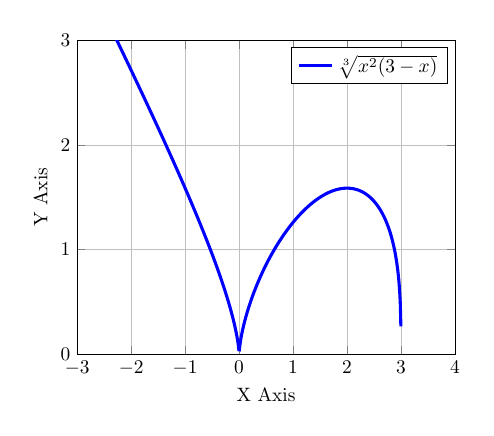
\begin{tikzpicture}[scale=0.7]
			\begin{axis}[
					xmax=4,
					xmin=-3,
					ymax=3,
					ymin=0,
					samples=1000,
					grid=major,
					xlabel={X Axis},
					ylabel={Y Axis},
				]
				\addplot[blue, ultra thick,domain=-5:5]{(x^2*(3-x))^(1/3)};
				\legend{$\sqrt[3]{x^2(3-x)}$}
			\end{axis}
		\end{tikzpicture}
		\caption{Final plot of curve from \pref{example}{exm-curve-sketching}}
		\label{sketch:exm-curve-sketching:1}
	\end{figure}
\end{exm}
